\chapter{Organisation}
\label{ch:Organisation}
A well-defined organisation, through structure, roles, and logic diagrams, ensures an efficient and great working environment during the project.
Hence, this chapter will dive deeper into each component, bringing together the greater picture of this organisation.

\section{Organisational Breakdown Structure}\label{sec:orgbreakdown}
Clearly establishing organisational and technical roles within the team is of paramount importance, since it will introduce a solid work division and communication between team members. 
Supported by the Organisational Breakdown Structure (OBS) in \Cref{fig:organogram}, the responsibilities and direct communication lines can be easily retrieved.
Additionally, the initials of each team member have been added to their role as well, showing that each member has at least one organisational and one technical role.
These can also be retrieved from the first page, which states the names, initials, and student numbers of each team member.
This division can be seen by the blue organisational department of the OBS, while the red area represents the technical department.
Moreover, the only two members to work in both departments of the OBS are the Quality Assurance Officer (QAO) and Systems Engineer (SE), for the sake of quality assurance. 
These two members work in great communication, both leading their own quality assurance process, which can be deduced by the red \enquote{QA}-squares in the OBS.
The QAO works closely with the Software Manager (SM) and Documents Manager (DM), while the SE works narrowly with the CAD Manager (CADM), to ensure a coordinated quality assurance process, which is a rather large task.
One more important feature to take away from the OBS is the approach to the organisational backbone of the team, which consists of the QAO, SE, and Project Manager (PM).
This triangular backbone ensures the smooth work flow during the project, while evenly dividing the vastly different workloads.
Each role will be further explained in the next subsections.

%A clear division of roles and responsibilities is of paramount importance for a functional working environment, hence this chapter establishes all organisational and technical roles each member of the team has. This will be illustrated by an organogram in \Cref{fig:orgbreakdownstruc}, and the responsibilities of each role are defined in \Cref{sec:org-roles}, as this will keep the organogram as organised and concise as possible. Moreover, the initials of each team member can be seen in each role, clarifying and simplifying the organogram. Every member of the team should at least be responsible for one organisational and one technical role, to ensure an equal and smooth workload.

\begin{figure}[ht]
    \centering    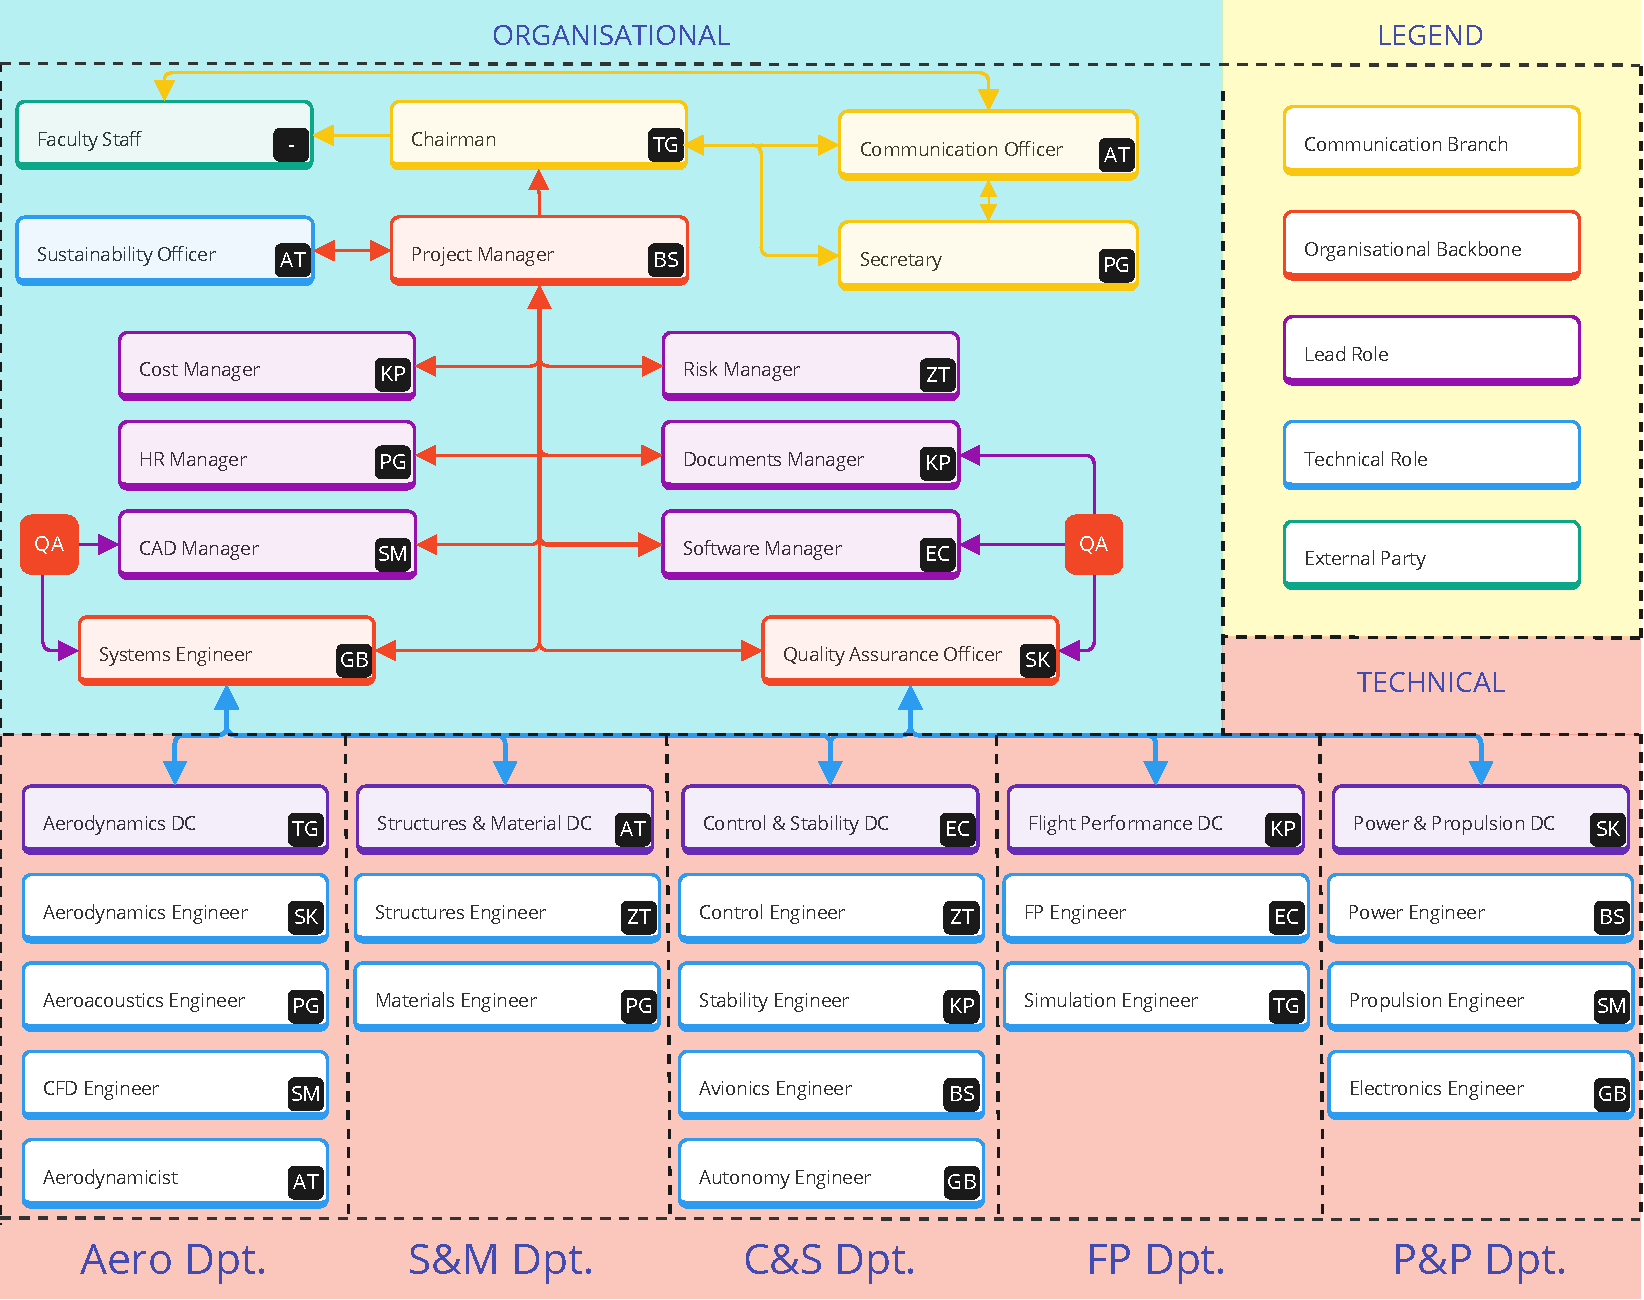
\includegraphics[width=1.0\linewidth]{figures/Organogram.pdf}
    \caption{Organisational breakdown structure}
    \label{fig:organogram}
\end{figure}

\subsection{Organisational Roles}\label{sec:org-roles}
 As the organisational roles are presented in \Cref{fig:organogram}, each role's responsibilities are further specified:

\textbf{Project Manager (PM)}: The PM can be seen as the coordinator, responsible for managing, planning and leading the team~\cite{dsePMSESlides1}.
The PM also defines, in consensus with the team, the proper procedures and organisation that must be followed, as well as closely monitoring the process and its adherence to the Gantt Chart (Appendix).

\textbf{Chairman}: As can be deduced from \Cref{fig:organogram}, the Chairman establishes the communication in the group, as it is in direct contact with external parties, the PM, and the communication branch.
The chairman is also responsible for leading the meetings and ensuring clear and efficient communication while adhering to the communication guidelines.

\textbf{Secretary}: The Secretary shall be responsible for administrative tasks, such as taking meeting notes and providing them in a proper document, as well as establishing meeting agendas for the Communication Officer.

\textbf{Communication Officer (CO)}: The CO is the only member, aside from the Chairman, to be in direct contact with the external parties, however with a greater emphasis on online communication.
The CO provides a clear meeting agenda in time to the external parties of interest, preferably through an Outlook meeting invitation.

\textbf{Sustainability Officer (SO)}: As the team deeply cares about its sustainable footprint, the SO will act as a gatekeeper for the team's sustainability.
Moreover, for each deliverable, the SO shall be responsible for reporting on the sustainability perspective of the document.

\textbf{Quality Assurance Officer (QAO)}: As earlier stated, the QAO and SE realise effective management of both the organisational and technical departments of the team.
Therefore, the QAO and SE shall always be in close contact, also in ensuring a well-organised quality assurance process. 
Both manage their own side of quality assurance while clearly communicating with each other.
The QAO is the main responsible role however, thus reporting to the PM. 
Moreover, the QAO establishes a clearly defined proofreading process, which is to ensure a smooth quality assurance process.

\textbf{Systems Engineer (SE)}: While also responsible for the quality assurance process, the SE is mainly in charge of effective workflow between technical departments, in order to meet the project's objectives.
The SE adheres to Systems Engineering by evaluating the team's systems and, where necessary, implementing improvements, thus be responsible for monitoring the total Systems Engineering perspective of the team.
As stated earlier, the SE shall be in close contact with the QAO, to ensure a smooth quality assurance process.

\textbf{Documents Manager (DM)}: The DM is responsible for the adherence of all documents to the standards set by the team, ensuring all the documents are of great scientific quality.
The DM shall accommodate a smooth document validation process, by keeping a well-organised archive of documents used, as well as the correct use of literature and references by the team.
The DM will also report to the QAO its progress and adherence to project guidelines, for the sake of the quality assurance process.
It is also the person responsible for handing in all the necessary deliverables on time.

\textbf{Software Manager (SM)}: The SM is responsible for the development, implementation, and maintenance of all software systems.
It shall manage the software written and used during the project, whilst meeting all technical specifications and operational requirements.
The SM also reports to the QAO its progress and adherence to project guidelines, for the sake of the quality assurance process.

\textbf{Computer-Aided Design Manager (CADM)}: The CADM is responsible for the fluent and effective use of CAD software during the project.
It is considered to be organisational, as can be seen from \Cref{fig:organogram}, although it does work together with several technical roles during the project.
The CADM is responsible for the management of the CAD technicians, thus ensuring conformance to industry standards and regulations, and shall report to the SE its progress and adherence to project guidelines, for the sake of the quality assurance process.

\textbf{Cost Manager (CM)}: The CM is in charge of the planning, monitoring, and controlling of project costs, as well as the development of budgets and maintenance.
When encountering problems, the CM shall be in close contact with the organisation's backbone.

\textbf{Risk Manager (RM)}: The RM coordinates the identification, assessment, analysis, and handling of the risk management of the team, both organisational and technical.
It provides a clear risk plan in order to tackle risks during the project, and monitors the adherence of the Systems Engineering during the risk analysis.

\textbf{Human Resources Manager (HRM)}: Although the HR is typically also externally oriented, the team chose this project's HRM to be solely internally focused, as at this stage, that is of greater importance.
The HRM oversees and ensures a well-defined HR allocation, realising smooth performance and development of the team during the project.
The HRM also ensures a safe working environment and great team member relations.

\subsection{Technical Roles}\label{sec:technical-roles}
The departments and their workload have been established by the OBS in \Cref{fig:organogram}.

The five technical departments of this project are \textbf{Aerodynamics}, \textbf{Structures \& Materials}, \textbf{Control \& Stability}, \textbf{Flight Performance}, and \textbf{Power \& Propulsion}.
Each department has its own Department Chief (DC), which shall ensure the proper division of tasks, while being able to meet deadlines.
Moreover, the expected workload of each department can be deduced by the amount of engineers put at each department. 
In order to ensure quality and efficient work, the departments are divided to conform to the team members' interests and expertise:

\textbf{Aerodynamics department}: The department is coordinated by the Aerodynamics DC and consists of an Aerodynamics, Aero-acoustics, and CFD Engineer, each having expertise in the matter.
As well as an Aerodynamicist who looks at the project more from a theoretical standpoint.

\textbf{Structures \& Materials department}: As this department only consists of a DC and two other engineers, hence those a Structures and Materials Engineer.

\textbf{Control \& Stability department}: This department has the highest workload together with Aerodynamics due to the complex flight dynamics that come with transformative wing concepts.
Besides the DC, the department consists of a Control, Stability, Avionics, and Autonomy Engineer, since the team deems these areas the most challenging for the department.

\textbf{Flight Performance department}: Since this department is rather small due to the expected workload, it consists of a Flight Performance and Simulation Engineer, as well as a coordinating DC.

\textbf{Power \& Propulsion department}: The last department consists of a DC, Power, Propulsion, and Electronics Engineer, all divided upon expertise and interest.

\section{Project Logic Diagrams}
In this section, the Logic Diagrams used in the organisation of the project shall be presented.
In order to complete a multidisciplinary project involving multiple people working in parallel at the same time, it is crucial to use tools such as a Work Flow Diagram (WFD), Work Breakdown Structure (WBS) and a Gantt chart in order to ensure completion in a timely manner.

\subsection{Work Flow Diagram}
\label{subsec:WorkFlowDiagram}
To facilitate the project planning, a Work Flow Diagram (WFD) was produced at the beginning of the project. In this diagram, all of the significant milestones and deliverables are illustrated, and the necessary activities that have to be performed during the project are mentioned.
%One crucial aspect that can be easily shown with the help of the workflow diagram is the %relationship between different modules (or milestones) that are part of the project.
%Using this method, it is easier to understand the flow of iterative activities, leading to %better planning, which can take iterations into account.
The diagram shows the sequence and iterative relations between the six main phases of the project and some lower-level tasks. Alongside the project phases, the responsible person, the total and throughput time are presented with a unique identifier. Furthermore, the inputs and outputs of the different project stages are highlighted in the diagram. To improve readability and enable easier understanding, the elements are colour-coded and referenced in the legend. The current version of the WFD can be found in the Appendix.

%In order to better illustrate the flow of the project, the project is split into six phases %(modules), and the flow between these phases, as well as the deliverables, is shown in a reduced %WFD that shall be included at the top of each of the two pages which showcase the project flow.
%Afterwards, each of the phases shall be presented in further detail through the presentation of %the inputs and outputs, as well as the constituent elements and their interrelations.
%Lastly, in order to improve readability and enable easier understanding, the elements are colour-%coded and referenced in the legend.



\subsection{Work Breakdown Structure}
\label{subsec:WorkBreakdownStructure} 
The work breakdown structure (WBS) is a fundamental tool in the context of project management.
The WBS is derived from the WFD and showcases all the phases of a project, broken down to a very high level of detail.
Particularly, it assigns each task that needs to be performed to some workers, also indicating the time needed to complete it. 
% It is a very complete tool that of course needs to be updated with the progress of the project since some unforeseen circumstances might have happened that changed the initial planning.
% Additionally, due to a better understanding of the project, the final phases can be further detailed in order to enable more precise planning.

In order to produce this diagram, firstly the total hour count to complete the project has been calculated.
Thereafter, these hours have been divided between the macro-phases of the project development, allocating hours with respect to the expected complexity of the phases.
Once this has been done, the macro phases are subdivided into the different sub-phases that characterise them.
For example, in the detailed design sub-phase the implementation of a 3D model is included.
These sub-phases are then broken down further till a sufficient level of detail is reached, such that the tasks can not be divided further. \\
Another important element of the WBS is assigning the expected time for each task as well as the responsible person for it.
The expected time can, however, be divided into effort and throughput time, where the effort is the total man-hours in order to complete a task while the throughput time is the time spent by each person to perform the task.
The diagram can be seen on the following page; for a better understanding, a mock box has been provided, explaining the meaning of each element.
As a final remark, in the diagram, phase 1 is not present as the planning was being made during phase 1.

\subsection{Gantt Chart}
\label{subsec:GanttChart}

A Gantt chart was made from the tasks of the WBS; in contrast, the Gantt chart features dependencies of the tasks.
In the Appendix, the full Gantt chart can be found.
In phase five, the detailed design phase, it can be seen that concurrent engineering is used.
Phases 5.1 to 5.4 run in parallel instead of in succession. After the first week of phase five, phase 5.5, the implementation of the 3D model will start, which will also run in parallel with the other phases.
From the gantt chart is can be seen that phase 6 starts before phase 5 ends, this is because there is a deadline for the design of the poster.
The initials of the team members are once again used to show responsibilities.
For the tasks during the first week of phase five some people are working partially on a task, this is indicated by "Initials[50\%]".


